\chapter{Étude du spectre discret de H au moyen de la résolvante}
% 192  II - ETUDE DU SPECTRE DISCRET DE H AU MOYEN DE LA RESOLVANTE
\section{Introduction}
Après avoir étudié, avec les états stationnaires de collision, la
partie continue du spectre du hamiltonien, nous passons maintenant à l'étude
de la partie discrète de ce spectre.

Soient $|$ i $>$ les états propres discrets, d'énergie E$_\mt{i}$ d'un hamiltonien H$_0$
\[
\tag{1}\mt{H}_0\;|\;\mt{i}>=\mt{E}_\mt{i}\;|\;\mt{i}>
\]
Ajoutons à ce hamiltonien une perturbation V. Il devient
\begin{center}
H = H$_0$ + V
\end{center}
Appelons $|\;\lambda>$ , les états propres également discrets de H, d'énergie E$_\lambda$
\[
\tag{2}\mt{H }|\;\lambda>=\mt{E}_\lambda\;|\;\lambda>
\]

Nous allons étudier comment les états $|\;\lambda>$ et les énergies E, se déduisent des
états $|$ i $>$ et des énergies E$_\mt{i}$.

Le traitement que nous donnons, du spectre discret est entièrement basé
sur l'utilisation de la résolvante, et présente par suite une grande analogie fomelle
avec celui du spectre continu présenté dans le chapitre précédent; il nous
permet par ailleurs d'établir des résultats qui nous serviront pour l'étude des
états instables.

Nous commençons par rappeler rapidement quelques propriétés de la résolvante ( \S B). Puis, nous étudions le cas d'un niveau non dégénéré de H$_0$ (\S C), ce qui
nous permet d'établir plusieurs résultats intéressants : (développement de Wigner-Brillouin des états propres et des énergies). Nous abordons ensuite le cas de 2
niveaux dégénérés ou quasidégénérés (\S D) et appliquons les résultats obtenus à
l'étude quantitative des transitions atomiques faisant intervenir l'absorption ou
l'émission de plusieurs quanta du champ électromagnétique (\S E).

% 193 
\section{La résolvante G(z)}% B
\subsection{Définitions}% 1

Appelons respectivement G(z)$=\frac{1}{\mt{z}-\mt{H}}$ et G$_0$(z)$=\frac{1}{\mt{z}-\mt{H}_0}$
les résolvantes des hamiltoniens H et H$_0$. Leurs éléments de matrices sont des fonctions
analytiques admettant pour pôles les valeurs propres des spectres discrets de H$_0$ et de
H, E$_\lambda$ et E$_\mt{i}$

\subsection{Relations entre G(z) et l'opérateur d'évolution U(t)}% 2
Rappelons simplement la relation (51) du \S 5 :
\[
\tag{3}\mt{U}(\mt{t})=\frac{1}{2\mt{i}\pi}\ \int_\mt{C}\mt{e}^{-\mt{i}\frac{\mt{Et}}{\hbar}}\mt{ G(E) dE}
\]
Le contour c est représenté par la figure ci-dessous\begin{center}
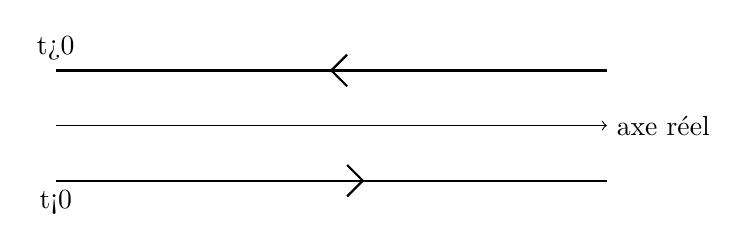
\begin{tikzpicture}
\draw [->] (-3.5,0) -- (3.5,0) node [right]{axe réel};
\draw [thick] (3.5,0.7) -- (-3.5,0.7) node [above]{t>0};
\draw [thick] (0.2,0.9) -- (0,0.7) -- (0.2,0.5);
\draw [thick] (3.5,-0.7) -- (-3.5,-0.7) node [below]{t<0};
\draw [thick] (0.2,-0.9) -- (0.4,-0.7) -- (0.2,-0.5);
\end{tikzpicture} \end{center}
Dans le cas où t > 0, il suffit d'intégrer sur l'axe du demi-plan supérieur; si
t < 0, on intègre sur l'axe du demi-plan inférieur


\subsection{Relation entre G et G$_0$}% 3

Rappelons que de la relation entre opérateurs
\[
{\mt{A}}-\frac{1}{\mt{B}}=\frac{1}{\mt{B}}(\mt{B}-\mt{A})\frac{1}{\mt{A}}
\]
on déduit la relation
\[
\frac{1}{\mt{Z}-\mt{H}}=\frac{1}{\mt{Z}-\mt{H}_0}+\frac{1}{\mt{Z}-\mt{H}_0}\mt{V}\frac{1}{\mt{Z}-\mt{H}}
\]
Soit
\[
\tag{4}\mt{G(Z)}=\mt{G}_0\mt{(Z)}+\mt{G}_0\mt{(Z) V G(Z)} \hspace{2cm} \mt{(formule 53, chap. 5)}
\]
qui permet d'obtenir par itération le développement :
\[
\mt{G(Z)}=\sum_{\mt{n}=0}^\infty\mt{G}_0\mt{ (V G}_0)^\mt{n}
\]
% 194
\section{Cas d'un niveau non dégénéré a de H$_0$. Etude de G$_0$(E) = $<$ a $|$ G(E) $|$ a $>$}% C
Soit $|$ a $>$, un état propre non dégénéré du hamiltonien H$_0$
d'énergie E$_\mt{a}$.

Nous allons voir que si l'on connaît l'action sur $|$ a $>$ de la résolvente G(E) et en particulier l'élément de matrice $<$ a $|$ G(E) $|$ a $>$, on est capable
d'en déduire, tout au moins \ul{théoriquement}, le spectre \ul{complet} des états propres
et des énergies du hamiltonien H. Pratiquement, on peut en déduire le développement
en série de la perturbation de l'état propre qui tend vers $|$ a $>$ lorsque
la perturbation tend vers zéro (ainsi que celui de son énergie).

L'avantage de la théorie présentée ici est d'obtenir des formules
rigoureuses, les approximations n'étant faites qu'à la fin des calculs.
\subsection{Première expression de G$_\mt{a}$(E)}% 1
La quantité fondamentale est $<$ a $|$ G(E) $|$ a $>=$ G$_\mt{a}$(E) dont nous pouvons
tout de suite donner une expression simple à l'aide de la relation de fermeture
$\sum_\lambda\;|\;\lambda><\lambda\;|\;=1$ :
\[
\tag{6}<\mt{a}\;|\;\mt{G(E)}\;|\;\mt{a}>\;=\;<\mt{a}\;|\;\frac{1}{\mt{E}-\mt{H}}\;|\;\mt{a}>\;=
\sum_\lambda\frac{|<\mt{a}\;|\;\lambda>|^2}{\mt{E}-\mt{E}_\lambda}
\]
On voit tout de suite sur l'expression (6) que les E$_\lambda$, du spectre discret sont les
pôles, de résidu $|<\mt{a}\;|\;\lambda>|^2$ de G$_\mt{a}$(E) (sauf si $<\mt{a}\;|\;\lambda>\;=$ 0). On peut donc dire
qu'en général, les valeurs propres de H sont les zéros de (G$_\mt{a}$(E))$^{-1}$.

{\footnotesize (La relation de fermeture $\sum_\lambda\;|\;\lambda><\lambda\;|\;=1$ doit évidemment porter sur les états du
spectre discret \ul{et} les états du spectre continu de $\mc{H}$. Seules les énergies propres
E$_\lambda$ du spectre \ul{discret} correspondent à des \ul{pôles} de la résolvante. Nous verrons plus
tard que le spectre continu $\mc{H}$ correspond à une "coupure" de la résolvante G(z)
Il est sous-entendu dans la suite de ce chapitre que les valeurs propres E$_\lambda$ envisagées sont des valeurs
propres du \mt{spectre discret} et nous n'exprimerons dans les relations de fermeture que les sommations sur les 
états discrets étant bien entendu
qu'il faut éventuellement y ajouter une sommation sur les états du spectre continu.)}

% 195 
Calculons maintenant l'élément de matrice $<$ b $|$ G(E) $|$ a $>$, $|$ b $>$
étant un état quelconque autre que $|$ a $>$ : on a de même
\[
\tag{7}<\mt{b}\;|\;\mt{G(E)}\;|\;\mt{a}>=\sum_\lambda\ \frac{<\mt{b}\;|\;\lambda><\lambda\;|\;\mt{a}>}{\mt{E}-\mt{E}_\lambda}
\]
Lorsque E $\to$ E$_\lambda$, les relations (6) et (7) permettent d'écrire
\[
\mt{G}_\mt{a}(\mt{E})=\frac{|<\mt{a}\;|\;\lambda>|^2}{\mt{E}-\mt{E}_\lambda}
\]
\[
<\mt{b}\;|\;\mt{G(E)}\;|\;\mt{a}>\ \sim\ \frac{<\mt{b}\;|\;\lambda><\lambda\;|\;\mt{a}>}{\mt{E}-\mt{E}_\lambda}
\]

On en déduit que l'expression $\frac{<\mt{b}\;|\;\mt{G(E)}\;|\;\mt{a}>}{\mt{G}_\mt{a}(\mt{E})}$
reste finie et tend vers $\frac{<\mt{b}\;|\;\lambda>}{<\mt{a}\;|\;\lambda>}$ :
\[
\tag{8}\frac{<\mt{b}\;|\;\mt{G(E}_\lambda)\;|\;\mt{a}>}{\mt{G}_\mt{a}(\mt{E}_\lambda)}=
\frac{<\mt{b}\;|\;\lambda>}{<\mt{a}\;|\;\lambda>}
\]
Les $|$ b $>$ formant un système complet, on a encore
\[
\tag{9}\lim_{\mt{E}\to\mt{E}_\lambda}\frac{1}{\mt{G}_\mt{a}(\mt{E})}\;\mt{G(E)}\;|\;\mt{a}>=
\sum_\mt{b}|\;\mt{b}>\lim_{\mt{E}\to\mt{E}_\lambda}
\frac{<\mt{b}\;|\;\mt{G(E}_\lambda)\;|\;\mt{a}>}{\mt{G}_\mt{a}(\mt{E}_\lambda)}
\]
\[
=\sum_\mt{b}|\;\mt{b}>\frac{<\mt{b}\;|\;\lambda>}{<\mt{a}\;|\;\lambda>}=
\frac{1}{<\mt{a}\;|\;\lambda)>}\;|\;\lambda>
\]
Enfin la connaissance de G$_\mt{a}$(E) nous permet grâce à (3) de calculer
\[
<\mt{a}\;|\;\mt{U(t)}\;|\;\mt{a}>\;=\frac{1}{2\mt{i}\pi}\int_\mt{c}\mt{G}_\mt{a}\mt{(E) e}^{-\mt{i}\frac{\mt{Et}}{\hbar}}\mt{ dE}
\]
qui représente l'amplitude de probabilité pour que le système étant dans l'état $|$ a $>$
à l'instant t = 0 y soit encore à l'instant t > 0. t étant positif le contour d'intégration est le suivant :
\begin{center}
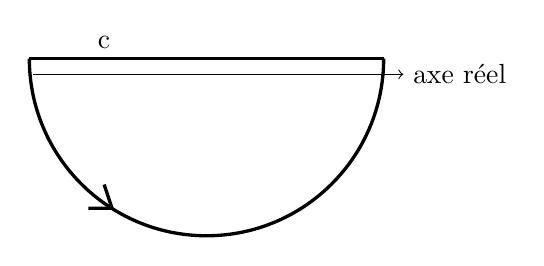
\begin{tikzpicture}
\draw [->] (-2.2,-0.2) -- (2.5,-0.2) node [right] {axe réel};
\draw [very thick] (-2.25,0) -- (2.25,0);
\draw [very thick] (-2.25,0)  arc (180:360:2.25);
\draw [very thick] (-1.5,-1.9) -- (-1.2,-1.9) -- (-1.3,-1.6);
\draw (-1.3, 0) node [above] {c};
\end{tikzpicture}
\end{center}
%%%%196 
et on a :
\[
\tag{10}<\mt{a}\;|\;\mt{U(t)}\;|\;\mt{a}>\;=\sum\mt{Res}\left[\mt{G}_\mt{a}\mt{(E) e}^{-\mt{i}\frac{\mt{Et}}{\hbar}}\right]
\]
\[
=\sum_\lambda|<\mt{a}\;|\;\lambda>|^2\mt{ e}^{-\mt{i}\frac{\mt{E}_\lambda\mt{t}}{\hbar}}
\]
La relation (10) que nous venons d'établir à l'aide de la résolvante est d'ailleurs
évidente : l'état $|$ a $>$ qui s'écrit à l'instant t = 0
\[
|\;\mt{a}>\;=\sum_\lambda|\;\lambda>|<\lambda\;|\;\mt{a}>
\]
devient, à l'instant t : $\sum_\lambda|\;\lambda>|<\lambda\;|\;\mt{a}>\mt{e}^{-\mt{i}\frac{\mt{E}_\lambda\mt{t}}{\hbar}}$
et l'amplitude de probabilité pour que le système soit dans l'état $|$ a $>$ à l'instant t est bien
\[
=\sum_\lambda|<\lambda\;|\;\mt{a}>|^2\mt{ e}^{-\mt{i}\frac{\mt{E}_\lambda\mt{t}}{\hbar}}
\]
\subsection{Définition des opérateurs F et R}% 2
Les relations (8) et (9) nous conduisent à définir un nouvel opérateur, F(E), par l'identité :
\[
\tag{11-a}<\mt{b}\;|\;\mt{G(E)}\;|\;\mt{a}>\;=\;<\mt{b}\;|\;\mt{F(E)}\;|\;\mt{a}><\mt{a}\;|\;\mt{G(E)}\;|\;\mt{a}>
\]
où encore
\[
\tag{11-b}<\mt{b}\;|\;\mt{F(E)}\;|\;\mt{a}>\;=\frac{<\mt{b}\;|\;\mt{G(E)}\;|\;\mt{a}>}{<\mt{a}\;|\;\mt{G(E)}\;|\;\mt{a}>}
\]
L'opérateur F(E), d'après (8), n'a pas de singularité lorsque E $\to$ E$_\lambda$, et on a évidemment l'égalité
\[
\tag{12}<\mt{a}\;|\;\mt{F(E)}\;|\;\mt{a}>\;=1
\]
$|$ b $>$ formant un système complet, nous pouvons de même définir l'action de F(E) sur $|$ a $>$ :
\[
\tag{13}\mt{F(E)}\;|\;\mt{a}>\;=\frac{1}{\mt{G}_\mt{a}\mt{(E)}}\;\mt{G(E)}\;|\;\mt{a}>
\]
et d'après (9)
\[
\tag{14}\mt{F(E}_\lambda)\;|\;\mt{a}>\;=\frac{1}{<\mt{a}\;|\;\lambda>}\;|\;\lambda>
\]

%%%%197 
L'opérateur F(E) est donc l'opérateur qui, lorsque E $=$ E$_\lambda$, transforme l'état propre discret $|$ a $>$ de H$_0$, en état propre discret | $\lambda$ > de H.

Appelons maintenant R(E) l' opérateur défini par son action sur le
vecteur $|$ a $>$ :
\[
\tag{15}\mt{R(E)}\;|\;\mt{a}>\;=\mt{V F(E) }|\;\mt{a}>
\]
R$_\mt{a}\mt{(E)}$ est l'élément diagonal de R (E) :
\[
\mt{R}_\mt{a}\mt{(E)}=\;<\mt{a}\;|\;\mt{ R(E) }|\;\mt{a}>
\]
\subsection{Deuxième expression de G$_\mt{a}\mt{(E)}$}% 3
Nous sommes maintenant en mesure d'établir une deuxième expression
rigoureuse, mais plus condensée de G$_\mt{a}\mt{(E)}$.
De (4), (11) et (15), on déduit :
\[
\mt{G}_\mt{a}\mt{(E)}=\frac{1}{\mt{E}-\mt{E}_\mt{a}}+\frac{1}{\mt{E}-\mt{E}_\mt{a}}\;<\mt{a}\;|\;\mt{V G(E) }|\;\mt{a}>
\]
\[
=\frac{1}{\mt{E}-\mt{E}_\mt{a}}+\mt{G}_\mt{a}\mt{(E)}\frac{1}{\mt{E}-\mt{E}_\mt{a}}\;<\mt{a}\;|\;\mt{V F(E) }|\;\mt{a}>
\]
\[
=\frac{1}{\mt{E}-\mt{E}_\mt{a}}+\mt{G}_\mt{a}\mt{(E)}\frac{1}{\mt{E}-\mt{E}_\mt{a}}\;\mt{R}_\mt{a}\mt{(E)}
\]
Soit
\[
\mt{G}_\mt{a}\mt{(E)}=\frac{1}{\mt{E}-\mt{E}_\mt{a}-\mt{R}_\mt{a}\mt{(E)}}
\]
L'expression (16) est rigoureuse. Les valeurs propres de H étant Les zéros de
(G$_\mt{a}$(E))$^{-1}$, le spectre de H est donc fourni par l'équation \ul{implicite}
\[
\tag{17}\mt{E}_\lambda-\mt{E}_\mt{a}=\mt{R}_\mt{a}\mt{(E}_\lambda)
\]
D'où le nom d'\ul{opérateur shift} donné à R(E) : ses éléments diagonaux dans l'état
$|$ a $>$, pris pour E = E$_\lambda$ représentent la différence entre E$_\lambda$ et E$_\mt{a}$.

% 198 —
\ul{Remarque} : L'équation implicite (17) fournit \ul{théoriquement toutes} les énergies
discrètes du hamiltonien H, et non pas uniquement, comme on pourrait le croire,
l'énergie E$_\alpha$, de l'état $|\;\alpha>$ qui tend vers $|$ a $>$ lorsque V $\to$ 0.

Cependant, pour ce niveau $|\;\alpha>$, le déplacement R$_\mt{a}$(E$_\alpha) =$ E$_\alpha$ - E$_\mt{a}$
sera une quantité petite lorsque V sera petit et on pourra en donner des
expressions approchées intéressantes. L'équation (17) est donc surtout \ul{pratiquement} utile pour le niveau d'énergie E$_\alpha$ qui tend vers E$_\mt{a}$ lorsque V $\to$ 0.
\subsection{Calcul de F(E) $|$ a $>$}%4
Appelons P$_\mt{a}=|\;\mt{a}><\mt{a}\;|$ le projecteur sur l'état $|$ a $>$ et
Q$_\mt{a}=1-$P$_\mt{a}$ le projecteur complémentaire.

Nous pouvons écrire
\[
\mt{F(E)}\;|\;\mt{a}>\;=\;|\;\mt{a}>\;<\mt{a}\;|\mt{ F(E) }|\;\mt{a}>+\sum_{\mt{b}\neq\mt{a}}\;|\;\mt{b}>\;<\mt{b}\;|\mt{ F(E) }|\;\mt{a}>
\]
\[
=\;|\;\mt{a}>+\mt{ Q}_{\mt{a}}\;\mt{F(E)}\;|\;\mt{a}>
\]
\[
=\;|\;\mt{a}>+\;\frac{1}{\mt{G}_{\mt{a}}\mt{(E)}}\mt{Q}_{\mt{a}}\;\mt{G(E)}\;|\;\mt{a}>
\]
Soit, en remplaçant G(E) par G$_0\;+$ G$_0$VG  et en remarquant que Q$_\mt{a}$ G$_0\;|$ a $>\;=0$ :
\[
\mt{F(E)}\;|\;\mt{a}>\;=\;|\;\mt{a}>\;+\;\frac{1}{\mt{G}_{\mt{a}}\mt{(E)}}
\frac{\mt{Q}_{\mt{a}}}{\mt{E-}-\mt{H}_0}\;\mt{V G(E)}\;|\;\mt{a}>
\]

D'où, finalement, compte tenu de (13) :
\[
\tag{18}\mt{F(E)}\;|\;\mt{a}>\;=\;|\;\mt{a}>\;+\;
\frac{1}{\mt{E}-\mt{H}_0}\;\mt{Q}_{\mt{a}}\mt{ V F(E)}\;|\;\mt{a}>
\]
qui s'écrit pour E $=$ E$_\alpha$
\[
\tag{19}\mt{F(E}_\alpha)\;|\;\mt{a}>\;=\;|\;\mt{a}>\;+\;
\frac{1}{\mt{E}_\alpha-\mt{H}_0}\;\mt{Q}_{\mt{a}}\mt{ V F(E}_\alpha)\;|\;\mt{a}>
\]
Or F(E$_\alpha$) $|$ a $>$ est, d'après (1), proportionnel à $|\;\alpha>$. (19) est donc une
équation "intégrale" reliant entre eux les vecteurs propres de H et de H$_0$ et
présente une grande analogie avec l'équation de Lippmam Schwinger reliant les
états propres de collision $|\;\psi_\mt{i}^\pm>$ et les états propres $\phi_\mt{i}$, de l'énergie cinétique T :

% 109

Si V est petit, on peut résoudre l'équation (19) par itération : on obtient

le développement de Yigner-Erillouin

Il faut remarquer que dans ce développement l'énergie perturbée figure au
dénominateur (contrairement au développement classique de Rayleigh-Schrüdinger )e

Le projecteur a fait que les somnations intermédiaires se font sur
des états autres que | a > : les dénominateurs sont de la forme  si
V est suffisamment petit, E , est petit et les termes en ne
divergent pas.

L'équation (18) permet théoriquement de calculer tous les états propres de H, mais on voit ainsi que c'est uniquement l'état | a > que l'on peut
atteindre par un calcul de perturbation.

5°) Calcul de R, (E) :

\subsection{}%
De (18) et (15) on déduit

\[
\tag{21}=
\]
que l'on peut écrire de façon opératorielle :

\[
\tag{22}=
\]
étent bien entendu que les deux membres agissent sur 

%%%%— 200 —

Remarque : Notons ici l'analogie qui existe entre l'opérateur shift R(E) et la
matrice de réaction en théorie des collisions,

Nous avons en effet, d'après (15)

ce qui, compte tenu de l'analogie déjà notée entre |  > et  |  >,
est l'analogie de l'équation

Nous pouvons maintenant effectuer un développement par itération de l'équation (22) :

ce qui nous donne le développement de R, (E) :

\[
\tag{23}=
\]

Ce développement ne pourra converger que si R(E) est suffisamment petit, donc
notamment pour E = E

Compte tenu de l'équation (17), on obtient alors le développement de
Wigner-Brillouin de l'énergie perturbée :

\[
\tag{24}=
\]

Tout comme dans le développement (20), l'énergie perturbée apparaît au dénominateur, mais pour les mêmes raisons, aucun dénominateur ne peut s'annuler si la

perturbation est suffisamment petite.

%%%%- 201 
En remplaçant de proche en proche dans les dénominateurs l'énergie
perturbée É par le développement (24) lui-même, on peut obtenir aux ordres
successifs le développement de Rayleiph-Schrüdinger, qui est explicite, mais
moins simple,

Faisons à titre d'exemple le calcul jusqu'au 3e ordre :

Jusqu'au 2e ordre inclus, le développement (2) reste valable, le
remplacement de E, par E, dans le terme du 2e ordre introduisant ure correction au 3e ordre : on a en effet, en posant

D'où le développement de Rayleigh-Schrôdinger au 3e ordre :
\[
\tag{25}=
\]
L'expression (22) de R(E) est une expression implicite. Nous allons maintenant
donner une forme explicite de R qui pourra être utile pour certeines applications. (22) peut s'écrire

ou

Soit

et en utilisant l'identité :

%%%%

\[
\tag{26}=
\]

\[
\tag{27}=
\]


\[
\tag{28}=
\]


\[
\tag{29}=
\]

% 202 —

il vient :

Utilisons à nouveau l'identité

dans l'expression (26); on obtient

, commute avec ; donc avec 

On peut donc commuter  et  dans le dernier terme du
développement (27). On fait alors apparaître le produit  et le dernier terme est nul.
D'autre part, on peut dans l'avant-dernier terme, en remarquant que  écrire
On obtient enfin, en multipliant les deux membres de (27) à gauche par

Etant bien entendu que dans (28), les deux membres sont des opérateurs agissant

sur 
On a en particulier :

Si on revient à la définition de

l'équation (28) conduit à l'équation que l'on aurait pu établir directement :

% 203

\[
\tag{30}=
\]
\[
\tag{31}=
\]

qui, pour , s'écrit

équation qui présente une grande analogie avec la forme explicite de
l'équation de Liprpmann-Schwinger :

 
\section{}
D, Cas de deux niveaux | a > et | b > dégénérés où quasi-dégénérés.

\subsection{}%
1°) Position du problème :

Nous allons maintenant envisager le cas où deux des niveaux d'énergie, a et b, du hamiltonien non perturbé  sont dégénérés où très voisins l'un
de l'autre, c'est-à-dire tels que leur différence d'énergie est très faible devant
celles qui les séparent de tous les autres niveaux.

Energie

L'introduction de la perturbation V va en général perturber fortement
les niveaux a et b et lever la dégénéréscence.

% 204
Les quantités intéressantes à calculer vont être 
 soit encore en appelant , le projecteur sur la multiplicité
dépénérée , la matrice , L'étude de ces quantités va nous permettre
de calculer les nouveaux niveaux d'énergie et les nouveaux états propres.

L'étude de  est également intéressante pour une autre raison :
 permet en effet, grâce à la relation (3), de calculer la quantité
 qui représente l'amplitude de probabilité pour que le système étant
dans l'état non rerturbé a à l'instant t = O se trouve dans l'état non perturbé b à l'instant t.

L'étude de la probabilité de transition entre deux niveaux a et b
d'un hamiltonien H sous l'effet d'une perturbation V est un problème très
important en physique ;: il arrive que les niveaux de He dépendent d'un para
mètre  (ils Sont par exemple fonction du champ magnétique). Pour certaines
valeurs du paramètre, deux niveaux a et b de He se croisent. L'effet de la
perturbation V peut être spectaculaire en ces points de croisement, La probabilité de transition entre a et b induite par V passe par un maximum résonnant

en ces points. Nous en verrons un exemple important dans la suite.

Energie

% 205

Plutôt que d'étudier le théorie es perturbations dégénérées proprement dites, nous allons surtout insister sur l'étude des probabilités de
transition entre deux niveaux dégénérés de He Nous soulignerons d'ailleurs
au fur et à mesure les liens étroits qui existent entre ces deux problèmes,

. Afin de nous familiariser davantage eævec l'emploi de la résolvente,
nous allons tout d'abord envisager un ess très simple, que l'on peut traiter
rigoureusement jusqu'au bout et qui ne mécessite pas l'emploi de techniques
mathématiques aussi élaborées, ous allons envisager un problème à doux niveaux a et b couplés par une perturbation non diagonale V et nous montrerons
comment Les formules simples obtenues peuvent se généraliser au cas plus compliqué où il existe un grand nombre de niveaux.
\subsection{}
2°) Etude d'un cas simple (problème à deux niveaux :

Aprelons E et E les énergies des deux niveaux | a > et | b > en
l'absence de la perturbation. Après avoir éventuellement intégré dans  les
Éléments diagonaux de la perturbation V, le seul élément de matrice non nul de
 reste 

Calculons l'élément de matrice non diagonal de la résolvente 
nouveau La relation () :

Ecrivons à

et itérons-le au deuxième ordre :

On obtient

Ou encore

\[
\tag{32}=
\]

\[
\tag{33}=
\]

\[
\tag{34}=
\]

% 206 =

Soit

Nous sevons que les zéros de  représentent les énergies perturbées

qui sont donc les racines de l'équation du second degré

qui s'écrivent

Le calcul de l'élément de matrice Ga (E) nous a ainsi fourni au passage l'expression
des énergies perturbées, résultat que l'on aurait pu obtenir beaucoup
plus simplement dans ce cas en diagonalisant la matrice

La relation (32) peut s'écrire en fonction des énergies E, et E :

On en déduit l'amplitude de probabilité de transition
 étant le contour

% 201

\[
\tag{36}=
\]
\[
\tag{37}=
\]
\[
\tag{}=
\]
D'où
Résidus
On en déduit la probabilité de transition de l'état a à l'état b à l'instent t :

169
La formule (36) s'appelle la formule de Rabi

Faisons l'hypotnèse que la perturbation V est appliquée à un ensemble comportant un très
grand nombre de systèmes à deux niveaux a et b identiques
à celui que nous venons d'étudier et que le temps pendant lequel la perturbation
V est appliquée varie aléatoirement d'un système à l'autre, la probabilité pour
que l'interaction dure un temps compris entre t et t + dt étant égale à 
(r étant le temps caractéristique du processus aléatoire),

On obtient la probabilité moyenne de transition de l'état a vers l'état
b en moyennant sur le temps  On obtient

(en posant T =
ce qui, après un calcul simple, donne, compte tenu de (36),

%%%%
Supposons maintenant que les énergies non perturbées E et E varient linéairement
en fonction d'un paramètre . Nous avons représenté en
trait pointillé sur la figure ci-dessous ces deux niveaux qui se coupent en
un point I

 

 

Nous avons représenté en trait plein les niveaux perturbés E, et E qui
se repoussent, en formant ce qu'on appelle un anticroisement, constitué par les
deux branches d'une hyperbole centrée en I dont la distance des sommets est égale

% 209

Nous voyons sur la formule (37) que la probabilité moyenne de transition de L'état a à l'état b sous l'effet du couplage V passe par un maxirum
résonnant au point d'anticroisement I (tel que E = E

La forme de la raie de résonance est Lorentzienne. L'intensité à
résonance varie comme  pour les valeurs faibles de V (tant que
) et est donc d'autant plus srande que les niveaux E, et E se

Lorsque V augnentee

.repoussent pluse Elle se sature et tend vers 


dépend à la fois du temps

La largeur de le résonance, à
caractéristique d'interaction r = 1/7 et ce 1'intensité du couplage. Pour 
faibles valeurs de  la largeur  est sensiblement égale à l
ce qui correspond à la quatrième relation d'incertitude temps-énergie : l'interaction
durant un temps moyen T: l'énergpie non perturbée est conservée à
 près. Pour les fortes valeurs de V, la largeur est égale à 
distance des sommets de l‘hyperbole d'anticroisement:

Le problème classique que nous venons d'étudier est extrêmement si:
et pouvait être résolu sans faire appel à la résolvante. Il nous  cependant permis
de mettre en évidence un certain nombre de résultats très pénéraux : nous
avons vu comment l'introduction d'une perturbation non diegonale entre deux niveaux
dégénérés repousse des deux niveaux et lève la dégénéréscence et comment
l'anticroisement" ainsi créé peut être associé à une yésonance dans la probabilité
de transition entre les deux niveaux non perturbése

Les problèmes physiques sont en rénéral beaucoup plus compliqués : il
existe plus de deux niveaux et la perturbation V peut induire un couplage entre
a et bet des niveaux c autres que à et b. D'autre part, le couplage entre ies
niveaux a et b peut être plus compliqué et s'effectuer par l'intermédiaire d'au
tres niveaux.

Nous allons maintenant établir une formule riçoureuse généralisant

l'expression (32) de Gba et valable dans tous les cas. Nous appliquerons ensuite
cette formule à un exemple très important : celui des transitions 
sieurs quantas Nous obtiendrons alors pour les probabilités de transition des

formules généralisant (37).

%%%%
3°) Cas général : On
\subsection{}%
Crateurs F et R :
 étant le projecteur sur les états a et b, appelons d le projecteur complémentaire :

Nous avons vu que la rrandeur essentielle de notre théorie est la matrice

Afin de calculer , nous allons, en généralisant la méthode employée
pour le cas non dégénéré, définir deux opérateurs  et .
Nous définissons  par la relation
à : 
qui généralise (1-a).

Comme G(E) commute avec P, on a aussi
vu
\[
\tag{38-b}=
\]
qui généralise (11-b)
Remarque : Nous voyons d'après (38-b) que l'on a défini en fait non pas l'opérateur
F(E) mais l'opérateur
On déduit de (38-b)

\[
\tag{39}=
\]
qui généralise (12).

Nous définissons alors , par la relation

et nous appelons R(E) la projection de R(E) dans Le sous-espace a,b

% 211 

\[
\tag{43}=
\]

°) Calcul de G(E) :
\subsection{}%
Considérons à nouveau l'identité

on en déduit

et compte tenu de (38-a)

Soit en multipliant à gauche par , et en tenant compte du fait que
 et , commutent : .

L'équation (42) est une égalité entre opérateurs agissant à l'intérieur du
sous-espace . Elle signifie que, dans ce sous-espace, l'opérateur 

est l'inverse de , Or E - H R(E) est représenté par la matrice

G(E) est donc renprésenté par la matrice inverse et on trouve, après un calcul
simple : 

La formule (43) rigoureuse, généralise la formule (32). Afin de l'utiliser, i

nous faut être capable de calculer , et donc 

%%%%

\[
\tag{45}=
\]
\[
\tag{46}=
\]
\[
\tag{47}=
\]
5°) Calcul de 

\subsection{}%
Nous avons

ce qui, compte tenu de (39) et de (38-b), s'écrit

Remplaçons alors  par  il vient

et finalement

expression qui généralise (18).

De (44) et de (40), on déduit

expression qui généralise (21).

On peut déduire de (45) le développement de Wigner-Brillouin de R(E) :

Les sommations sur les états intermédiaires dans (46) font intervenir tous les
états autres que a et b et le développement pourra donc converger si on donne
à E des valeurs assez voisines de a et
On peut enfin donner à (E) une forme explicite analogue à (28) et qui
se démontre de la même manière

%%%%- 213 
\section{}
E. Application : théorie des transitions à plusieurs quanta

Nous allons appliquer les résultats du paragraphe précédent aux
transitions à plusieurs quanta de radiofréquence entre les sous-niveaux
Zeeman d'un atome.

1°) Description. expérimentale ;

\subsection{}%
Considérons un niveau atomique de spin J = 1/2 et supposons que
par un procédé quelconque, nous puissions orienter le spin dans une direction donnée, le long de laquelle est appliqué un champ magnétique statique
B. Supposons que ce spin interagisse pendant un temps t avec un champ de
radiofréquence Ë cos $\omega$ t, linéaire, de pulsation $\omega$, orienté perpendiculairement à H. Supposons enfin que le système observé est constitué par un
grand nombre de spins indépendants, le temps d'interaction t avec le champ
de radiofréquence variant aléatoirement d'un spin à l'autre et que l'on me
sure la probabilité moyenne P de trouver le spin renversé à la fin de l'in
teraction (ces conditions expérimentales pourront par exemple être réalistes
sur un jet atomique orienté par un aimant de type Stern et Gerlach et passant
dans une région où règne le champ de radiofréquence perpendiculaire au champ
statique (ef fig. a). La variation du temps d'interaction entre le spin et
la radiofréquence est alors due à la dispersion des vitesses. On peut également envisager une orientation des spins par pompage optique longitudinal
d'une cellule de résonance placée dans un champ cos $\omega$t (fig. b). Le
temps d'interaction dépend alors de la relaxation des spins dans la cellule).
cos $\omega$
orientation

région d'inter- detection
action

Figure a Figure b

J.MH. WINTER - Thèse Paris 1958 (Anne Physe h, 1959, pe 745) of

 
% 214

Quel que soit le procédé expérimental utilisé, on constate que P
passe par un meximum résonnant lorsque la fréquence de Larmor dans le champ
magnétique  u$\omega$ = , (y raprort gyromagnétique), est égale à la fréquence
$\omega$ de la radiofréquence : il s'agit de le résonance magnétique classique ordinaire. Lorsqu'on augmente l'intensité de la radiofréquence, on constate que
la résonance  s'élargit et subit un déplacement vers les faibles valeurs du chemp H (shift de Bloch-Siegert) alors qu'il apparaît une nouvelle
résonance pour $\omega$, = $\omega$, Cette résonance subit à son tour un élargissement et
un déplacement, etc, On peut ainsi mettre en évidence tout un spectre impair
de raies de résonance magnétique qui apparaissent lorsque la fréquence de
Larmor est un multiple impair de la fréquence $\omega$ de la radiofréquence et qui
subissent des élargissements et des déplacements importants lorsque l'intensi
té de la radiofrédquence augmente. (cf figure ci-dessous)

Intensité croissante
de la radiofréquence

 $\omega$ 3$\omega$ 5$\omega$ 7$\omega$ $\omega$
Il est possible de donner une interprétation physique simple de ces
résonances : le champ de radiofréquence linéaire peut être décomposé en deux
composantes circulaires droite et gauche , et . Les résonances observées correspondent à des transitions entre les deux sous-niveaux Zeeman +1/2 et -1/2
par absorption d'un ou plusieurs photons de radiofréquence. La nécessité de

conserver à la fois l'énergie et le moment angulaire au cours de la transition

%%%%
fait que le nombre de photons intervenant est nécessairement impair : chaque
photon transportant une unité de moment angulaire le long de seul un
nombre impair d'entre eux permet d'induire des transitions ,

Ce raisonnement, qui justifie le spectre impair, ne nous pérmet cependant pas
de rendre compte des élarrissements @t déplacements observés, Nous allons pour
cela faire une théorie plus complète de ces transitions en traitant quantique

ment le champ de radiofréquence,

2°) Hamiltonien du système "spin-radiofréquence"

\subsection{}%

Orientons  le long de Oz et H le long de Ox.

Appelons a et a les onérateurs d'unnihilation et de création d'un
photon dans le mode du champ. Le hemiltonien du système combiné constitué par
le spin 1/2 couplé au champ de radiofréquence est constitué de trois termes :
$\alpha$) Le hamiltonien Zeeman du spin 1/2 :
$\beta$) Le hamiltonien du champ de radiofréquence : $\omega$

(en négligeant le terme 1/2 Hu ce qui est justifié étant donné -le très grand
nombre de photons contenus dans le champ de radiofréquence).

$\gamma$) Le hamiltonien d'interaction entre le spin et Le champ : 

Ce hamiltonien s'écrit classiquement.

% 216

Afin de traiter quantiquement H(t), rappelons que le potentiel
vecteur À du champ électromagnétique s'écrit

étant une somme portant sur les directions et polarisations des modes
dont les opérateurs d'annihilation et de création respectifs sont

Le champ magnétique  s'écrit

Dans le cas présent, un seul mode du champ est rempli, celui dont la polarisation
est parallèle à Ox et dont le module du vecteur d'onde

On peut donc écrire

étant Le vecteur unitaire Le long de Ox et « une constante de proportionnalité
réelle. Afin de se débarrasser de la constante imaginaire i, il est toujours
possible de faire sur la variable *un changement d'origine en posant

On en déduit :

La longueur d'onde du champ de radiofréquence est très grande et nous supposerons
que l'interaction avec les spins se fait sur des distances beaucoup plus courtes;
 on peut alors poser 

et 
Le hamiltonien  s'écrit alors

À étant une constante de proportionnalité,

% 217

\[
\tag{49}=
\]

Pour évaluer cette constante, nous devons faire une hypothèse sur
l'état quantique représentant le champ de radiofréquence classique.

Nous prendrons pour représenter Le champ l'état quantique se rapprochant le plus de l'état classique, c'est-à-dire un état cohérent de
Glauber | y > (cf Phys. Rev.131,1963,2766 ). Rappelons que cet état est tel
que les valeurs moyennes de l'énergie et du champ sont égales aux grandeurs
classiques correspondantes et qu'il s'obtient en faisant agir un opérateur

de déplacement  sur l'état représentant le vide | O > :

L'opérateur  se définit par son action sur les opérateurs  :

Rappelons enfin que le nombre moyen de photons contenu dans l'état |  >,
N est égal à .

D'après la propriété fondamentale de l'état |  > , la valeur moyenne’ dans cet état de
l'opérateur  doit être égale à la grandeur classique correspondante, Ho, :

or
% 218

Remarque : L'énergie du champ de radiofréquence est proportionnelle à y

\[
\tag{50-a}=
\]
\[
\tag{50-b}=
\]

(classiquemænt) et à N (quantiquement). $\omega$, est donc proportionnel à N.

C'est cette proportionnalité que traduit la formule (49) :

En conclusion : le hamiltonien du système "spin 1/2, champ de radiofréquence"

est
avec

avec
3°) Etude des niveaux d'énergie de
\subsection{}%
Le hamiltonien  admet pour énergies propres les énergies

les états propres étant les états |  > représentant le spin dans l'état
+ 1/2 le long de Oz en présence de n photons de radiofréquence,
Le diagramme d'énergie de , est représenté sur la figure ci-dessous en
fonction du champ magnétique 
Nous voyons que ce diagramme présente une infinité de croisements de
niveaux pour toutes les valeurs du champ H, telles que $\omega$, = nu (n entier positif)

%%%%- 219 
Le couplage  possède des éléments de matrice non nuls
entre les états tels que  et Un simple examen des niveaux
d'énergie montre alors que les niveaux qui se croisent aux points tels que
$\omega$, = (2n+l)$\omega$ sont connectés par la perturbation (à l'ordre Pn+1) alors que
les points de croisement tels que $\omega$, = 2n$\omega$ ne le sont à aucun ordre,

4°) Principe du calcul des formes de raie des transitions
\subsection{}%
Nous sommes donc, pour les croisements tels que $\omega$, = (2n+l$\omega$)
remenés à l'étude du \S D et nous pouvons prévoir une résonance dans la probabilité
de transition sous l'effet du couplage H, entre les deux niveaux non
perturbés qui se croisent. Afin de calculer les probebilités et les formes de
raie qui en résultent, il nous suffit d'appliquer les résultats résumés dans
les relations (43) et (37).

Pour calculer La probabilité de transition entre a et b, au point de croisement
des niveaux non perturbés a et b, il faut partir de l'expression rigoureuse (43)

à l'aide de laquelle on calcule. Et

puis

et enfin

Le calcul de  se fait par la méthode des résidus : nous avons vu (\S B) que
 admet pour pôles toutes les énergies propres discrètes E, du hamiltonien

 avec pour résidu .

% 220

\[
\tag{51}=
\]
\[
\tag{52}=
\]
Nous voyons tout de suite que les résidus les plus importants sont ceux pour
lesquels | $\lambda$ > = | a > ou | b >, | a > et | b > étant les états perturbés de
valeur propre E, et E, correspondant aux états non perturbés a et b. Tous
les autres résidus seront d'un ordre supérieur, | a > et | b > étant pratiquement
orthogonaux à tout état | $\lambda$ > autre que | a > ou | b >, Nous nous contenterons donc,
pour le calcul de  des deux résidus aux pôles E et E
qui sont donnés par les équations implicites

Nous nous bornerons de plus à un calcul de perturbation à l'ordre

le plus bas. Nous savons alors qu'il est possible de remplacer les énergies
perturbées E et E
l'énergie E correspondant au croisement des niveaux non perturbés E et E
par les énergies non perturbées, et en particulier par

Nous pouvons alors écrire

Nous obtenons alors pour  une expression explicite approchée analogue

à l'expression (32) à partir de laquelle nous pouvons, par les mêmes calculs,

déduire pour  une expression analogue à (37) :

Il nous suffit maintenant, afin de calculer les formes de raie des transitions
à plusieurs quante à l'ordre le plus bas de la perturbation, de nous placer au
point de croisement des niveaux non perturbés correspondant (u$\omega$, = (2n+1)u$\omega$) et
de calculer à l'ordre le plus bas où elles sont non nulles chacune des trois
quantités  à l'aide du développement en série de la perturbation (46).

% 221 
L'expression (52) fournit alors la forme de Fe et donne notamment l'intensité (qui dépend de ),
la largeur  et le déplacement radiatif Rate R(E) - AC (E) de la résonance, Nous allons prendre pour
exemple le cas des transitions à un quantum ($\omega$, = $\omega$) et à trois quanta

5°) Transition à un quantum : Shift de Bloch et Siegert
\subsection{}%
Nous allons prendre pour états | a > et | b > les états

Remarque : L'état du champ de rayonnement n'est pas un état | n >, mais une superposition cohérente d'états | n > autour d'une valeur moyenne N. Le caractère
cohérent du champ n'intervient pas dans l'étude de la probabilité de transition.
La dispersion relative du nombre de photons du champ  étant très
petite, tout se passe comme si l'état initial du champ était un état | n >
avec nv.

Les deux niveaux d'énergie correspondant aux états a et b se coupent
pour $\omega$. = $\omega$ et pour une énergie 

Nous avons $\omega$.

a) Calcul de 

D'après le développement (46), en remplaçant V par
$\omega$.

(d'après (49) )

% 222

B) Calcul de  et 

D'après (6), on a

Or le niveau  est relié au er ordre aux niveaux

et |  >, Le niveau intermédiaire dans le calcul de ,  doit être différent de | b >.
Ce ne peut donc être que |  > d' énergie $\omega$

On a donc
Qu

Ra (E) = <ntl = | 3 (ata*) | n+2,+ >< n+2,+ | 7 (ata*) | nt, >

et finalement, d'après (52), on trouve

Nous retrouvons les différentes propriétés de le transition à un quantum : la
$\omega$
largeur qui est égale à  pour les faibles valeurs de $\omega$, augmente lorsqu'on
augmente H et est proportionnelle à $\omega$ u$\omega$ pour les fortes valeurs

% 223

$\omega$

la résonance, centrée en  subit un déplacement radiatif en
 vers les faibles valeurs du champ : c'est le shift de Bloch et Siegert
dont nous avons donné ici un calcul particulièrement simple.

Lorsqu'on augmente  l'intensité à résonance croît en $\omega$ pour
les faibles valeurs de 

6°) Transition à trois quanta
\subsection{}%

Nous prenons pour états | a > et | b > les états

Les deux niveaux d'énergie correspondant se coupent pour $\omega$ et pour une

énergie .

Nous avons d'autre part $\omega$).

a) Calcul de 

La relation () nous montre que pour aller de 
il faut passer par deux états intermédiaires :
$\omega$

8) Calcul de  et 

Il s'effectue comme pour la transition à un quantum :

%%%%

Or le nivesu  est relié au premier ordre aux
niveaux , d'énergie  qui sont tous les deux différents

d'énergie $\omega$

de

On a donc

De même cn montre que
$\omega$
et finalement, d'après (52), on obtient

$\omega$
ou encore
%%%%
(54)nous fournit les principales propriétés de  transition à trois quantas :
la largeur de la résonance  qui tend vers  lorsque
$\omega$, tend vers zéro, est proportionnelle à $\omega$  lorsque $\omega$, devient suffisamment grande


.L'intensité à résonance croît en u$\omega$. Pour les faibles valeurs de

puis se sature.

Enfin la résonance, centrée en 

déplacement radiatif en $\omega$ vers les faibles valeurs du champ

. subit un

On peut très facilement calculer les formes de raie pour les transitions à (2n+1 quanta et trouver des formules analogues à (53) et (54),

On montrerait notamment que la résonance à (2n+1) quanta  une intensité
proportionnelle à H pour des valeurs suffisamment faibles de  une
largeur proportionnelle à x, (2n+1) (pour des valeurs pas trop faible de H.)
et subit un déplacement radiatif en H° vers les faibles valeurs du champ.

voulons

%%%%
